\documentclass[11pt]{jarticle}
\usepackage[dvipdfmx]{graphicx}
\usepackage[dvipdfmx]{color}
\usepackage{kcctd-report}
\usepackage{booktabs}
\usepackage{mathcomp}
\usepackage{array}
\usepackage{mathtools,amssymb}
\usepackage{siunitx}
\usepackage{multirow}
\usepackage{tabularx}
\usepackage{subcaption}
\usepackage{float}
\usepackage{listings,jvlisting}
\lstset{
	basicstyle={\ttfamily},
	identifierstyle={\small},
	commentstyle={\smallitshape},
	keywordstyle={\small\bfseries},
	ndkeywordstyle={\small},
	stringstyle={\small\ttfamily},
	frame={tb},
	breaklines=true,
	columns=[l]{fullflexible},
	numbers=left,
	xrightmargin=0zw,
	xleftmargin=3zw,
	numberstyle={\scriptsize},
	stepnumber=1,
	numbersep=1zw,
	lineskip=-0.5ex,
	tabsize=2
}
\renewcommand{\lstlistingname}{ソースコード}

\title{半導体加工技術と特性評価 pn接合の作製}
\adviser{西 敬生  教授}

\sdate{令和5年6月29日}
\edate{令和5年7月6日}
\fdate{令和5年7月11日}
\rdate{}

\grade{5}
\anumber{12}
\gnumber{B}
\name{河合 将暉}
\jname{
		岡田 晃空 川邊 愛貴 久戸 悠大 久米 椋翔
	  }
\comment{}
\begin{document}
\maketitle

\section{目的}
半導体素子を作成する上で最重要技術である不純物拡散によるシリコンPN接合作成技術を習得し、半導体素子や集積回路の作成技術に関する基本概念を得ることを目的とする.
\section{解説}
	\subsection{拡散}
		異種の粒子が異なった濃度分布で共存するとき,この混合系が熱平衡状態に近づこうとして起こる濃度分布一様化の過程を拡散という.
		拡散を原子の移動という立場から眺めてみると,原子が結晶欠損(穴)に異動するもの,格子間の本来結晶格子がとるべきではない位置へ移動するもの,複数の原子が互いの位置を入れ替えるものがある.
		拡散の過程では,これらが単独に,あるいは組み合わさって起こる.
	\subsection{半導体}
		抵抗率を$10^3~10^9\,\mathrm{\Omega cm}$の範囲に制御できる物質の総称.
		またこの半導体の電気的特性が光,磁気,熱など外部エネルギの影響を強く受ける.
		新聞紙上など,一般的に用いられている場合は,この半導体を材料に作られたICなどのデバイスを指している.
	\subsection{伝導型(p型,n型)}
		半導体中には,マイナスの電荷をもつ電子とプラスの電荷をもつ正孔が存在する.
		2つを合わせて``キャリア''と呼ぶ.
		電子が多い半導体をn型(negativeの頭文字),正孔が多い半導体をp型(positive)と呼ぶ
	\subsection{PN接合}
		p型とn型の半導体が``くっついた''部分に電圧を印加すると整流性が現れる.
	\subsection{ショットキー接触}
		p,nどちらかの半導体と,ある金属を接合させた場合も整流性が現れる.

\section{実験内容}
	\subsection{使用器具}
		\begin{table}[H]
		\begin{center}
		\caption{使用器具}
		\label{tab:used}
		\begin{tabular}{clllll} \toprule
		No&\multicolumn{1}{l}{機器名}&\multicolumn{1}{l}{型番}&\multicolumn{1}{l}{シリアルNo}&\multicolumn{1}{l}{備考}\\ \hline
		1&電気炉&&&\\
		2&ディップコーター&&&\\
		3&真空蒸着装置&&&\\
		4&ホットプレート&&&\\
		5&ジェットオーブン&&&\\
		6&定電圧電源&&&\\
		7&ディジタルマルチメータ&&&\\ \bottomrule
		\end{tabular}
		\end{center}
		\end{table}

	\subsection{実験方法}
		この実験は,拡散現象を利用してシリコン基板中に不純物を混入させ,pn接合を作成した.
		基板の表面からドナーもしくはアクセプタとなる物質を拡散によって混ぜ入れると,表面に近いほど濃度が高い不純物濃度分布となる.
		拡散させた不純物の濃度が基盤自体の不純物濃度に等しくなる深さの位置が,pn接合となる.
		つまり,不純物がアクセプタの場合,不純物混入を行った面がp型,逆側がn型のダイオードの構造となる.

		また,ダイオードを電気回路中に組み込むためには,当然のことながらこれと金属との接触が必要となる.
		しかしながら金属と半導体を単純に接触させると,p型半導体とn型半導体の接触時に作成するショットキー障壁が発生し,この接触部によって新たなダイオードができるので,意図する特性が得られなくなる.
		このため,金属半導体接合部の整流性を排除した抵抗性接触になるようにダイオードに電極を付ける.
		これは,ショットキー障壁の高さを下げるか,壁厚を薄くする(これによりトンネル効果により電流が多く流れるようになる)ことと半導体側のキャリア再結合速度を増大させることで実現できる.
		障壁の厚さは金属の仕事関数の大きさに,壁厚は半導体のキャリア濃度の高さに依存する.
		この実験では,金属の仕事関数を上げる(勢いよく半導体に付着させる)ために,蒸着法を用いた.
		\subsubsection{pn接合試料作成手順}
			\begin{enumerate}
				\item 酸化膜付SiウェーハをFine Crystl Cutterで$1\mathrm{cm} \time 2.5\mathrm{cm}$ぐらいにカット.
				\item ウェーハを洗浄
				\item ディップコータでレジストをウェーハの半分だけ塗布し,保護膜を形成.
				\item ウェーハをバッファードフッ酸の中に入れ,レジストがついていない部分だけ酸化膜エッチング
				\item レジストをアセトン1+第2プロパノール1の混合液とメタノールで除去
				\item P(リン)化合物が解けた不純物溶液を酸化物が除去されたSiウェーハ部分にディップコータで塗布した.
					  ここで,ディップコータからの引き上げ時間を1\,mm/sと0.1\,mm/sに分けて行い,0.1\,mm/sのウェーハ裏面にダイアモンドペンを用いて印付けを行った.
					  ウェーハ5枚のうち,1\,mm/sを3枚,0.1\,mm/sを2枚に分けて実験を行った.
				\item ホットプレート100~200$^\circ \mathrm{C}$,1分で溶液の乾燥.
				\item 電気炉内で焼成し不純物拡散(1000$^\circ \mathrm{C}$以上 30分)
				\item バッファードフッ酸による不純物ガラス,酸化膜のエッチング
				\item Al蒸着による電極形成
				\item ホットプローブ法によりpn判定で,不純物拡散の出来を確認
				\item 試料の保護のためのスライドガラスをガラス切りによって切断
				\item ロウにより,切断したスライドガラスと試料を接着
			\end{enumerate}
		\subsubsection{測定方法}
			\begin{enumerate}
				\item pn接合ダイオードの順方向・逆方向I−V特性\\
					\begin{enumerate}
						\item 市販のダイオードと電流計,電圧計,直流電圧電流源を接続し,順方向特性について測定した.
							  市販の整流用ダイオードの測定ではしきい電圧の約0.65V以下までは高抵抗素子として,電圧計は電源と並列で,電源は電圧源として測定した.
							  しきい電圧の約0.65V以下までは高抵抗素子として以上は,低抵抗素子として電圧計はダイオードと並列接続し,電源は電流源として測定した.
							  10\,mAになるまで測定した.
						\item 逆方向特性を測定する.20Vぐらいまで電圧を印加したときの電流を確認した.
					\end{enumerate}
				\item 作成したpn接合の順方向・逆方向I−V特性\\
					\begin{enumerate}
						\item 試料表面の電極に測定用針を接触させ,静特性を測定した.
						\item した試料と直流低電圧電流源,電圧計,電流計を接続し順方向のI‐V特性を測定した.
							  このとき,試料の内部抵抗が高いため,以下の全測定において電源は電圧源として使用した.
							  電流が1mAになるまで測定した.(内部抵抗が高いため,しきい電圧以上の電圧を印加する必要がある)
						\item 逆方向特性を測定した.
							  pn接合の降伏現象を確認したいが,内部抵抗が高いため急激な電流の増加は見られないがグラフ化すると傾きが異なるため判明する.
							  そのためグラフがしっかり描けるように測定点を多めにした.
					\end{enumerate}
			\end{enumerate}
\clearpage
\section{実験結果}
	\subsection{pn接合ダイオードの順方向・逆方向I−V特性}
		市販品のpn接合ダイオード素子に閾値以下の順方向電圧を印加したときのI‐V特性を表\refeq{tab:kiseipnunder}に示す.
		\begin{table}[H]
		\centering
		\caption{市販pn接合ダイオードの順方向I−V特性(閾値以下)}
		\label{tab:kiseipnunder}
		\begin{minipage}{0.4\columnwidth}
		\centering
		\begin{tabular}{SS} \toprule
			電圧 [mV] & 電流 [$\mathrm{\mu}$A] \\ \hline
			0.000 & 0.06 \\
			49.99 & 0.06 \\
			100.0 & 0.06 \\
			150.0 & 0.08 \\
			200.0 & 0.13 \\
			249.0 & 0.31 \\
			308.8 & 1.11 \\
			318.8 & 1.41 \\
			328.7 & 1.79 \\
			338.7 & 2.31 \\
			348.6 & 3.18 \\
			358.7 & 3.90 \\
			368.6 & 5.07 \\
			378.6 & 6.58 \\
			388.6 & 8.59 \\
			398.5 & 11.80 \\
			408.5 & 14.56 \\
			418.5 & 18.84 \\
			428.4 & 24.25 \\
			438.4 & 31.10 \\
			448.4 & 40.90 \\
			458.3 & 49.82 \\
			468.3 & 62.22 \\
			478.2 & 76.59 \\
			488.2 & 93.59 \\
			498.2 & 116.1 \\
			508.1 & 135.6 \\
			518.1 & 161.2 \\ \bottomrule
			
		\end{tabular}
		\end{minipage}
		\hspace{0.04\columnwidth}
		\begin{minipage}{0.4\columnwidth}
		\centering
		\begin{tabular}{SS} \toprule
			電圧 [mV] & 電流 [$\mathrm{\mu}$A] \\ \hline
			528.1 & 189.6 \\
			538.1 & 220.7 \\
			548.1 & 258.6 \\
			558.0 & 292.3 \\
			568.0 & 332.8 \\
			578.0 & 375.8 \\
			587.9 & 421.8 \\
			597.9 & 474.2 \\
			607.9 & 521.7 \\
			617.8 & 575.8 \\
			629.8 & 642.9 \\
			639.8 & 701.3 \\
			649.8 & 761.0 \\
			659.7 & 823.8 \\
			669.7 & 887.4 \\
			679.6 & 953.1 \\
			689.6 & 1020.2 \\
			699.6 & 1087.4 \\
			709.6 & 1157.6 \\
			719.5 & 1227.2 \\
			729.5 & 1299.5 \\
			739.4 & 1373.0 \\
			749.4 & 1447.1 \\
			759.4 & 1521.0 \\
			769.4 & 1596.2 \\
			779.3 & 1673.1 \\
			789.3 & 1751.4 \\
			799.3 & 1829.2 \\ \bottomrule
		\end{tabular}
		\end{minipage}
		\end{table}
		次に,市販pn接合ダイオードの順方向電圧印加時のI‐V特性を表\refeq{tab:kiseipnover}に示す.
		\begin{table}[H]
		\begin{center}
		\caption{市販pn接合ダイオードの順方向I−V特性(閾値以上)}
		\label{tab:kiseipnover}
		\begin{tabular}{SS} \toprule
			電流 [mA] & 電圧 [V] \\ \hline
			0.9996 & 0.5838 \\
			1.099 & 0.5883 \\
			1.199 & 0.5921 \\
			1.300 & 0.5958 \\
			1.400 & 0.5990 \\
			1.499 & 0.6022 \\
			1.599 & 0.6051 \\
			1.699 & 0.6077 \\
			1.799 & 0.6099 \\
			1.899 & 0.6122 \\
			1.999 & 0.6130 \\
			9.996 & 0.6900 \\
			19.989 & 0.7201 \\
			29.988 & 0.7371 \\
			39.984 & 0.7489 \\
			49.984 & 0.7579 \\
			59.96 & 0.7652 \\
			69.95 & 0.7712 \\
			79.94 & 0.7763 \\
			89.93 & 0.7806 \\
			99.93 & 0.7846 \\ \bottomrule
		\end{tabular}
		\end{center}
		\end{table}

		表\refeq{tab:kiseipnunder},\refeq{tab:kiseipnover}をまとめてグラフにしたものを図\refeq{fig:pnI-V}に示す.
		\begin{figure}[H]
		\centering
		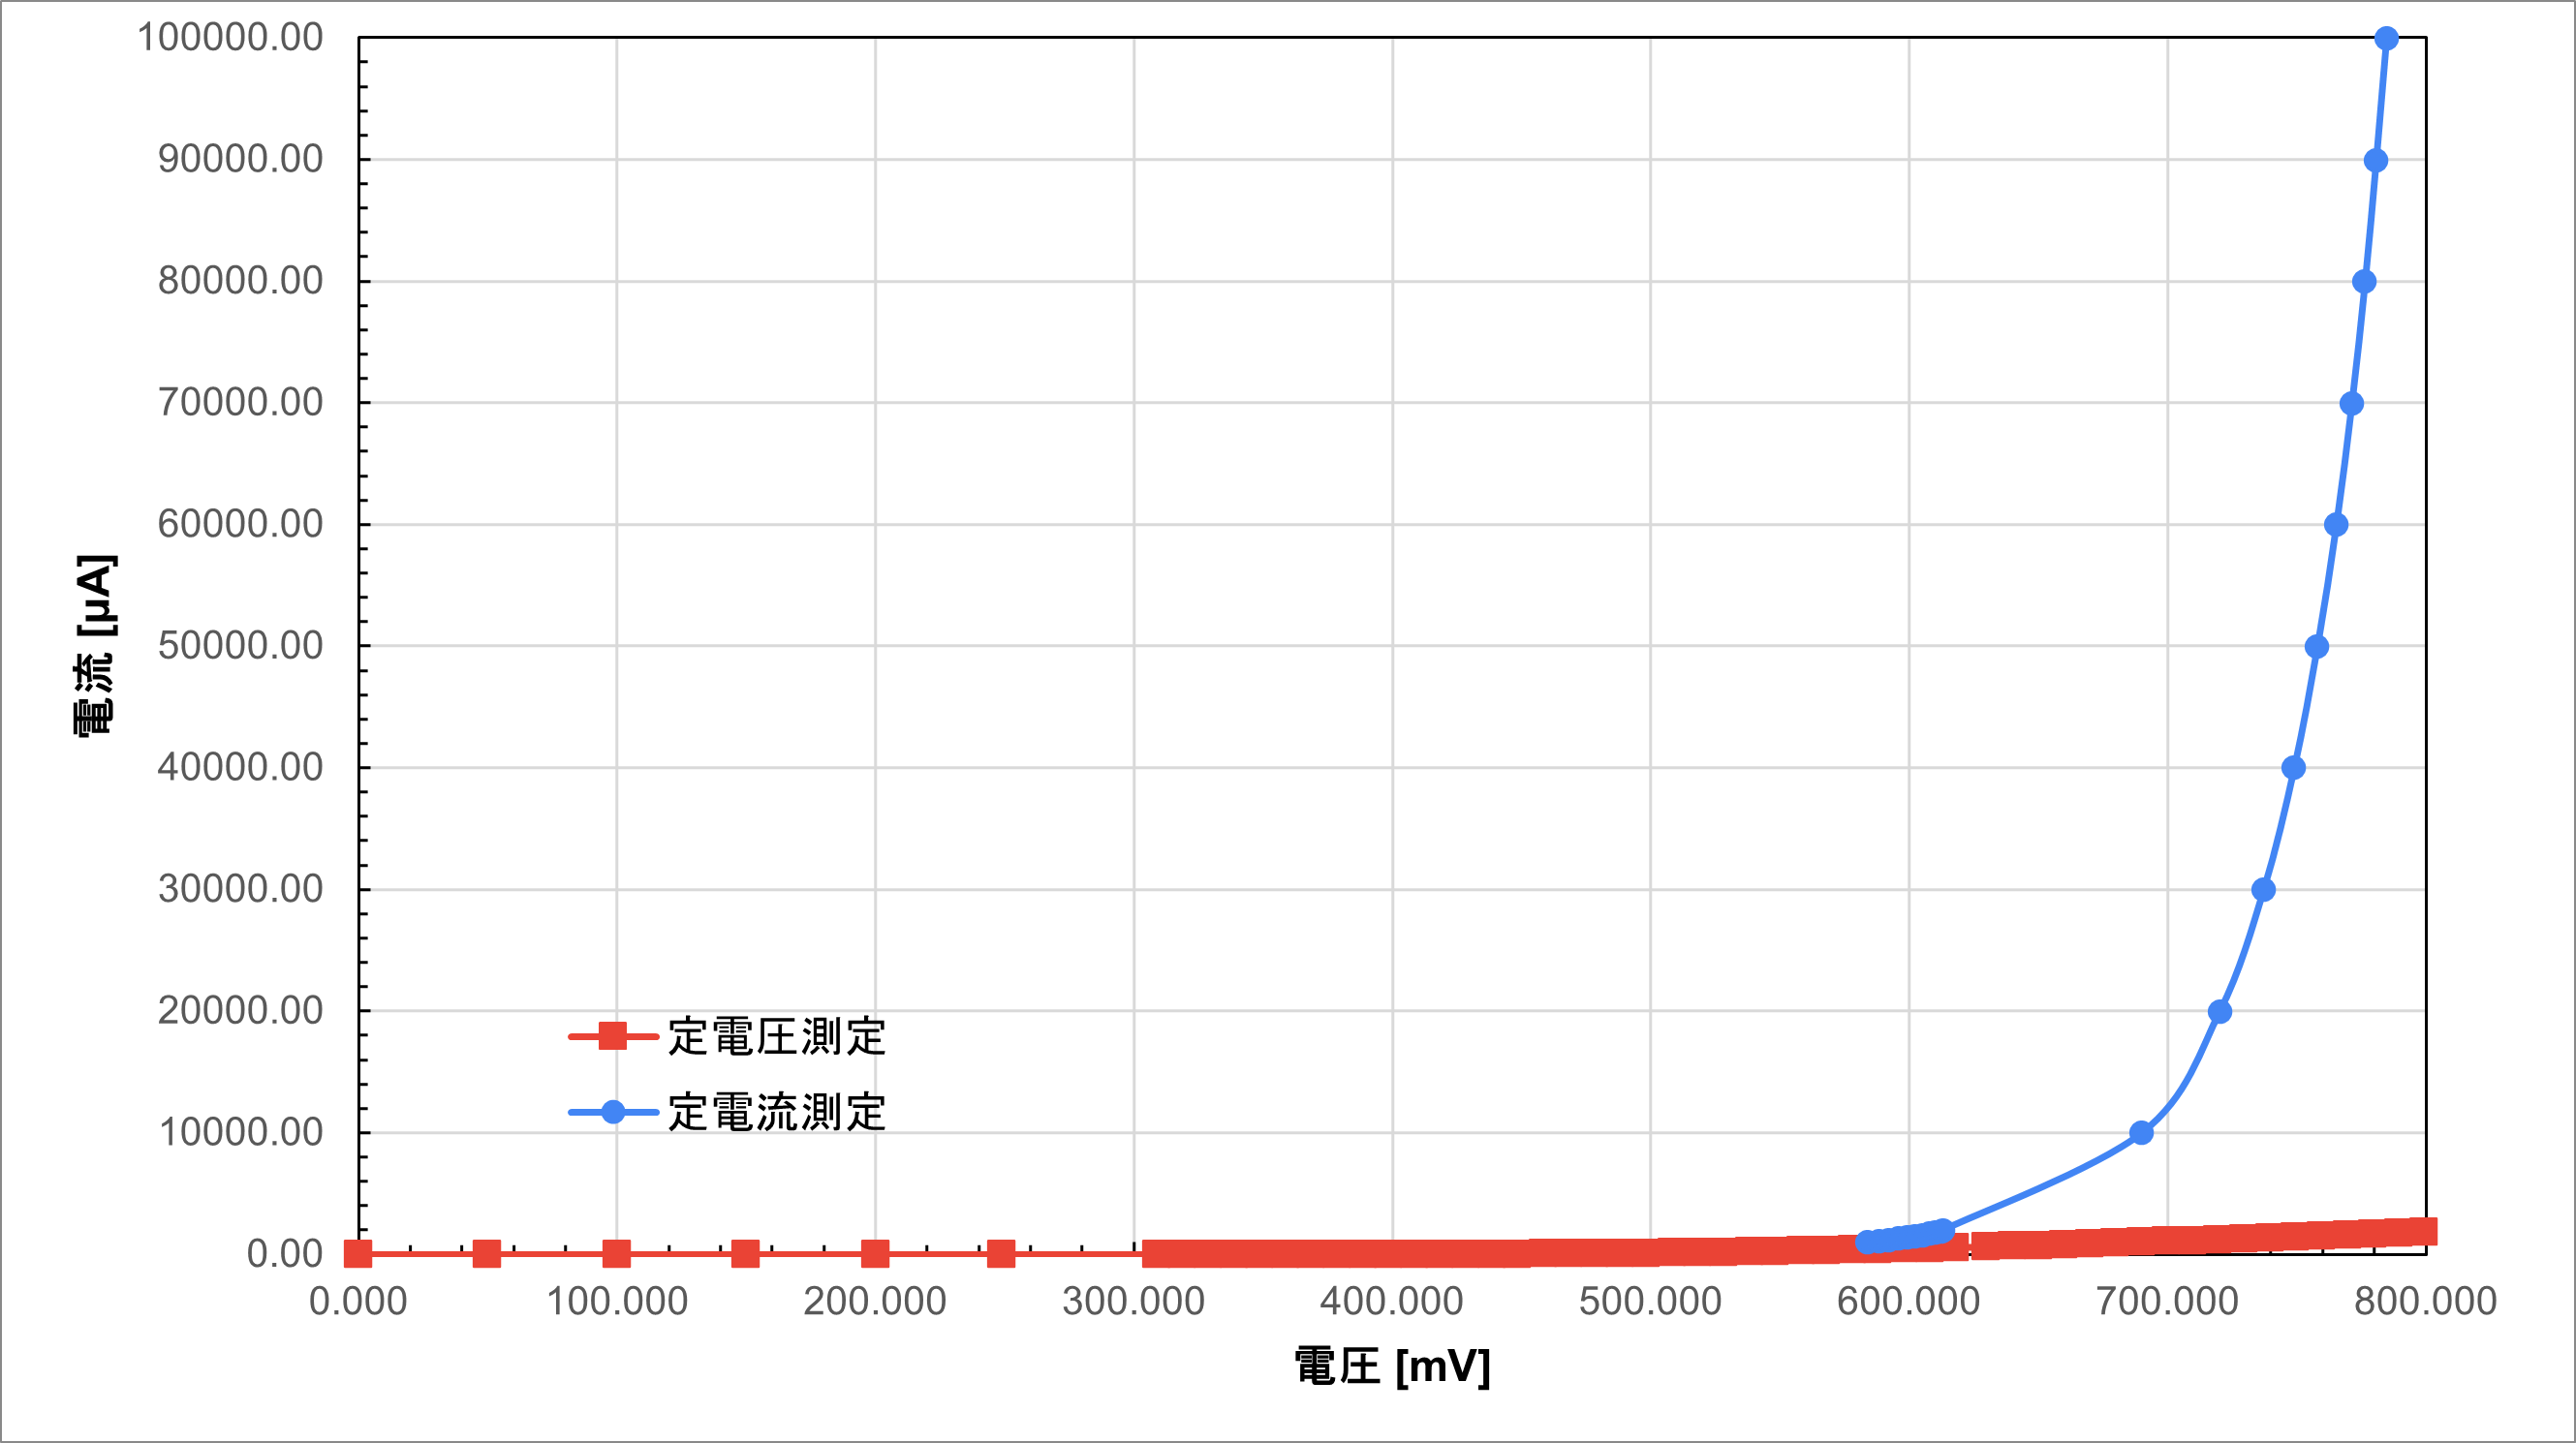
\includegraphics[width = 12cm]{figs/chart.png}
		\caption{市販pn接合ダイオード順方向電圧印加I‐V特性図}
		\label{fig:pnI-V}
		\end{figure}

		図\refeq{fig:pnI-V}より,定電流で測定したものは閾値以上でpn接合の2乗特性が現れており,急峻に電流が増加していることがわかる.
\clearpage
		市販品のpn接合ダイオード素子に逆方向電圧を印加したときのI‐V特性を表\refeq{tab:kiseipngyaku}に示す.
		\begin{table}[H]
		\begin{center}
		\caption{市販pn接合ダイオードの逆方向電圧印加I−V特性}
		\label{tab:kiseipngyaku}
		\begin{tabular}{SS} \toprule
			電圧 [mV] & 電流 [$\mathrm{\mu}$A] \\ \hline
			-0.640 & 0.06 \\
			-49.36 & 0.06 \\
			-99.30 & 0.06 \\
			-144.18 & 0.06 \\
			-199.06 & 0.06 \\
			-248.91 & 0.06 \\
			-298.78 & 0.06 \\
			-348.56 & 0.06 \\
			-448.31 & 0.06 \\
			-498.15 & 0.06 \\
			-548.1 & 0.06 \\
			-597.9 & 0.06 \\
			-649.8 & 0.06 \\
			-5000 & 0.06 \\
			-10000 & 0.06 \\
			-20000 & 0.06 \\
			-25000 & 0.06 \\ \bottomrule
		\end{tabular}
		\end{center}
		\end{table}
		表\refeq{tab:kiseipngyaku}より,25Vの逆方向電圧を印加しても電流は変化しなかった.
		ダイオードの整流性より,逆方向電圧を印加したときは電流が流れないことから正しく動作していることがわかる.

	\subsection{作成したpn接合の順方向・逆方向I−V特性}
		作成したpn接合のうち,簡易pn判定法としてホットプローブ法を用いて,pn判定を行った.
		その際に,pn接合ができているものはn型のときに0.017~0.02\,mV程度,p型の時に-0.5~-0.9\,mV程度の電圧を測定することができた.
		加工の際に1枚だけ1cm程度長いウェーハができたが,そのウェーハのpn判定ではp型の際に最大-1.4\,mVを測定することができた.
		
		また,電極間を測定して自然光による光起電力を測定すると,pn接合できているものは約200\,mV程度測定することができた.
		5枚のうち3枚が前述の程度で測定でき,ほかの2枚は光起電力が1.9\,mV程度で,pn接合ができていないと予想した.
\clearpage
		次に,pn接合ができている3枚のうち,引き上げ速度が1\,mm/sのウェーハに順方向電圧を印加したI‐V特性を表\refeq{tab:jisakupnjun1}に示す.
		\begin{table}[H]
		\begin{center}
		\caption{引き上げ速度1\,mm/sにおけるpn接合の順方向I−V特性1}
		\label{tab:jisakupnjun1}
		\begin{tabular}{SS} \toprule
			電圧 [V] & 電流 [μA] \\ \hline
			0.0000 & -71.95 \\
			0.1991 & -34.33 \\
			0.2191 & -14.50 \\
			0.2490 & -5.970 \\
			0.2988 & 23.95 \\
			0.3496 & 59.33 \\
			0.3995 & 88.90 \\
			0.4194 & 101.8 \\
			0.4394 & 115.8 \\
			0.4593 & 129.6 \\
			0.4793 & 143.6 \\
			0.4992 & 159.6 \\
			0.5191 & 176.2 \\
			0.5391 & 192.2 \\
			0.5590 & 209.6 \\
			0.5789 & 228.1 \\
			0.5989 & 246.7 \\
			0.7993 & 485.4 \\
			0.9996 & 808.2 \\ \bottomrule
		\end{tabular}
		\end{center}
		\end{table}

		表\refeq{tab:jisakupnjun1}をグラフにしたものを図\refeq{fig:pnjun1}に示す.

		\begin{figure}[H]
		\centering
		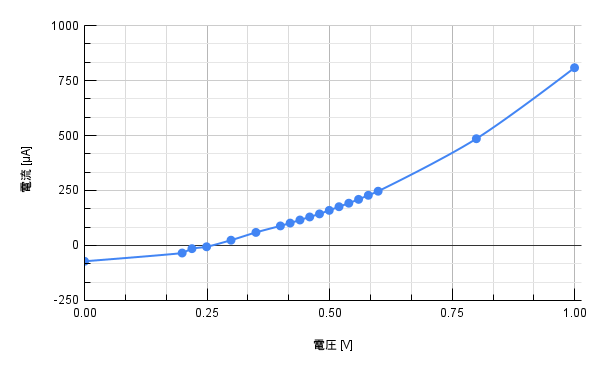
\includegraphics[width = 12cm]{figs/chart1.png}
		\caption{引き上げ速度1\,mm/sにおけるpn接合の順方向I−V特性図1}
		\label{fig:pnjun1}
		\end{figure}

		図\refeq{fig:pnjun1}より,おおよそ0.25~0.5\,Vで緩やかに増加していることがわかる.
\clearpage
		次に,同じウェーハに対して逆方向電圧を印加したときのI‐V特性を表\refeq{tab:jisakupngyaku1}に示す.
		\begin{table}[H]
		\begin{center}
		\caption{引き上げ速度1\,mm/sにおけるpn接合の逆方向I−V特性1}
		\label{tab:jisakupngyaku1}
		\begin{tabular}{SS} \toprule
			電圧 [V] & 電流 [mA] \\ \hline
			-0.0002 & -0.056 \\
			-0.9997 & -0.089 \\
			-2.000 & -0.103 \\
			-2.999 & -0.114 \\
			-3.999 & -0.142 \\
			-4.999 & -0.194 \\
			-5.199 & -0.220 \\
			-5.400 & -0.307 \\
			-5.599 & -0.407 \\
			-5.799 & -0.513 \\
			-6.001 & -0.623 \\
			-6.199 & -0.728 \\
			-6.400 & -0.841 \\
			-6.599 & -0.953 \\
			-6.800 & -1.072 \\
			-7.000 & -1.187 \\
			-8.000 & -1.845 \\
			-9.000 & -2.518 \\
			-10.00 & -3.208 \\ \bottomrule
		\end{tabular}
		\end{center}
		\end{table}

		表\refeq{tab:jisakupngyaku1}をグラフにしたものを図\refeq{fig:pngyaku1}に示す.
		\begin{figure}[H]
		\centering
		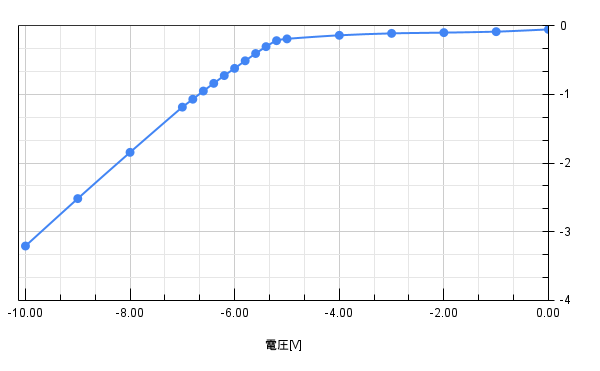
\includegraphics[width = 12cm]{figs/chart4.png}
		\caption{引き上げ速度1\,mm/sにおけるpn接合の逆方向I−V特性図1}
		\label{fig:pngyaku1}
		\end{figure}

		図\refeq{fig:pngyaku1}より,-5.0\,V付近で電流降伏が起きていることがわかる.
		ダイオードに高い逆方向電圧を印加するとアバランシェ破壊とツェナー破壊が起こり,電流が急激に降伏していると考えられる.
\clearpage
		もう1枚の引き上げ速度が1\,mm/sのウェーハに順方向電圧を印加したI‐V特性を表\refeq{tab:jisakupnjun2}に示す.
		\begin{table}[H]
		\begin{center}
		\caption{引き上げ速度1\,mm/sにおけるpn接合の順方向I−V特性2}
		\label{tab:jisakupnjun2}
		\begin{tabular}{SS} \toprule
			電圧 [V] & 電流 [mA] \\ \hline
			0.0000 & -52.45 \\
			0.1991 & -21.37 \\
			0.2499 & -0.820 \\
			0.2988 & 50.16 \\
			0.3496 & 138.6 \\
			0.3995 & 249.1 \\
			0.4493 & 379.3 \\
			0.4992 & 530.3 \\
			0.5490 & 695.8 \\
			0.5989 & 872.7 \\
			0.7993 & 1666.6 \\
			0.9997 & 2533.6 \\ \bottomrule
		\end{tabular}
		\end{center}
		\end{table}

		表\refeq{tab:jisakupnjun2}をグラフにしたものを図\refeq{fig:pnjun2}に示す.
		\begin{figure}[H]
		\centering
		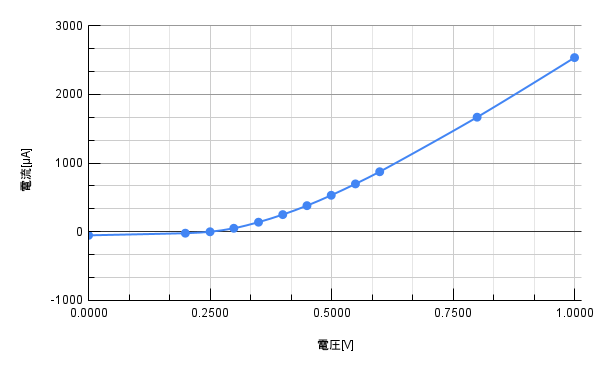
\includegraphics[width = 12cm]{figs/chart2.png}
		\caption{引き上げ速度1\,mm/sにおけるpn接合の順方向I−V特性図2}
		\label{fig:pnjun2}
		\end{figure}
		図\refeq{fig:pnjun2}より,0.35\,V付近で電流が増加し始め,その後は電圧に比例するように増加していることがわかる.
\clearpage
		同じウェーハに対して逆方向電圧を印加したときのI‐V特性を表\refeq{tab:jisakupngyaku2}に示す.
		\begin{table}[H]
		\begin{center}
		\caption{引き上げ速度1\,mm/sにおけるpn接合の逆方向I−V特性2}
		\label{tab:jisakupngyaku2}
		\begin{tabular}{SS} \toprule
			電圧 [V] & 電流 [mA] \\ \hline
			0.000 & -0.048 \\
			-1.000 & -0.062 \\
			-1.999 & -0.073 \\
			-2.999 & -0.111 \\
			-3.999 & -0.16 \\
			-4.499 & -0.226 \\
			-4.999 & -0.267 \\
			-5.500 & -0.337 \\
			-6.000 & -0.415 \\
			-7.000 & -0.588 \\
			-8.000 & -0.793 \\
			-9.000 & -1.016 \\
			-10.00 & -1.263 \\ \bottomrule
		\end{tabular}
		\end{center}
		\end{table}

		表\refeq{tab:jisakupngyaku2}をグラフにまとめたものを図\refeq{fig:pngyaku2}に示す.
		\begin{figure}[H]
		\centering
		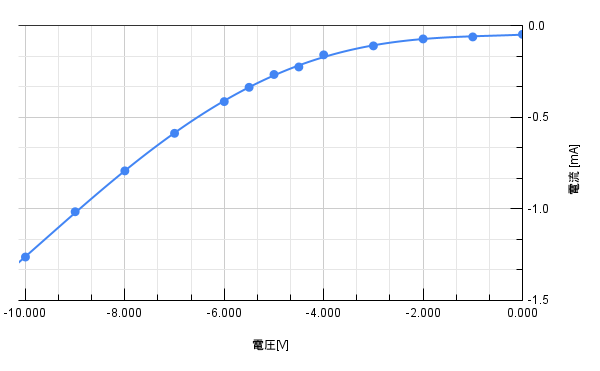
\includegraphics[width = 12cm]{figs/chart5.png}
		\caption{引き上げ速度1\,mm/sにおけるpn接合の逆方向I−V特性図2}
		\label{fig:pngyaku2}
		\end{figure}

		図\refeq{fig:pngyaku2}より,逆方向電圧を大きくするほど逆方向の電流が指数関数的に増加していることがわかる.
\clearpage
		引き上げ速度が0.1\,mm/sのウェーハに順方向電圧を印加したI‐V特性を表\refeq{tab:jisakupnjun0.1}に示す.
		\begin{table}[H]
		\begin{center}
		\caption{引き上げ速度0.1\,mm/sにおけるpn接合の順方向I−V特性}
		\label{tab:jisakupnjun0.1}
		\begin{tabular}{SS} \toprule
			電圧 [V] & 電流 [μA] \\ \hline
			0.002 & -40.89 \\
			0.1991 & -2.120 \\
			0.2090 & 0.07 \\
			0.2191 & 6.950 \\
			0.2290 & 17.13 \\
			0.2390 & 24.75 \\
			0.2490 & 35.18 \\
			0.2589 & 41.82 \\
			0.2689 & 53.44 \\
			0.2789 & 65.74 \\
			0.2888 & 78.69 \\
			0.3197 & 123.1 \\
			0.3397 & 158.1 \\
			0.3596 & 193.7 \\
			0.3796 & 231.1 \\
			0.3995 & 272.7 \\
			0.5989 & 768.8 \\
			0.7993 & 1373.1 \\
			0.9997 & 2033.4 \\ \bottomrule
		\end{tabular}
		\end{center}
		\end{table}

		表\refeq{tab:jisakupnjun0.1}をグラフにまとめたものを図\refeq{fig:pnjun0.1}に示す.
		\begin{figure}[H]
		\centering
		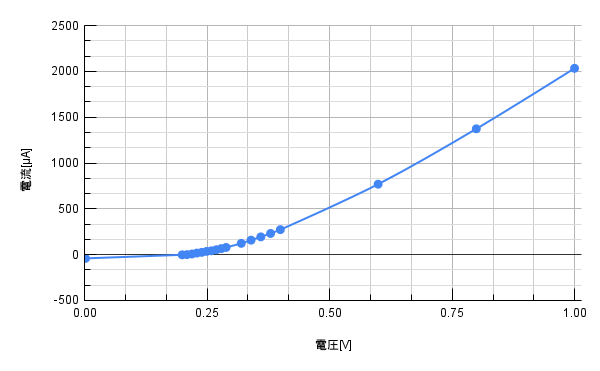
\includegraphics[width = 12cm]{figs/chart3.png}
		\caption{引き上げ速度0.1\,mm/sにおけるpn接合の順方向I−V特性図}
		\label{fig:pnjun0.1}
		\end{figure}
		図\refeq{fig:pnjun0.1}より,0.25\,V付近で電流が増加し始め,その後は電圧に比例して電流が増加していることがわかる.
\clearpage
		同じウェーハに対して逆方向電圧を印加したときのI‐V特性を表\refeq{tab:jisakupngyaku0.1}に示す.
		\begin{table}[H]
		\begin{center}
		\caption{引き上げ速度0.1\,mm/sにおけるpn接合の逆方向I−V特性}
		\label{tab:jisakupngyaku0.1}
		\begin{tabular}{SS} \toprule
			電圧[V] & 電流[mA] \\ \hline
			0.000 & -0.0490 \\
			-1.000 & -0.0750 \\
			-2.000 & -0.1200 \\
			-3.000 & -0.1760 \\
			-4.000 & -0.2660 \\
			-5.000 & -0.3770 \\
			-5.499 & -0.4430 \\
			-6.001 & -0.5200 \\
			-6.500 & -0.5910 \\
			-7.000 & -0.6810 \\
			-8.000 & -0.8750 \\
			-9.000 & -1.265 \\
			-10.00 & -1.835 \\ \bottomrule
		\end{tabular}
		\end{center}
		\end{table}

		表\refeq{tab:jisakupngyaku0.1}をグラフにまとめたものを図\refeq{fig:pngyaku0.1}に示す.
		\begin{figure}[H]
		\centering
		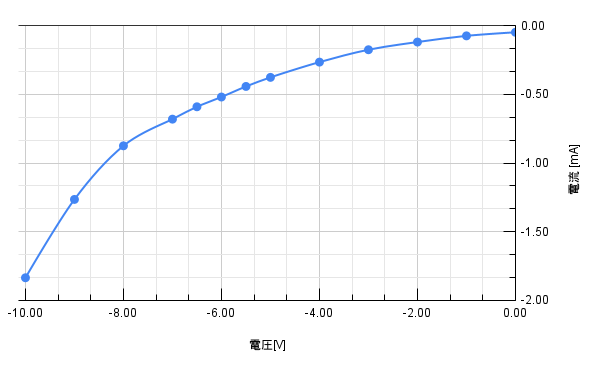
\includegraphics[width = 12cm]{figs/chart6.png}
		\caption{引き上げ速度0.1\,mm/sにおけるpn接合の逆方向I−V特性図}
		\label{fig:pngyaku0.1}
		\end{figure}
		図\refeq{fig:pngyaku0.1}より,0~-8.0\,Vまでは緩やかに逆方向電流が増加しているが,それよりも大きい逆電圧ではより大きく傾いていることがわかる.
		これはアバランシェ破壊かツェナー破壊のどちらかが最初に起きていて,-8.0\,V以上の逆電圧で両方の破壊降伏が起きたと考えられる.

\section{考察}
	\subsection{pn判定}
		今回の実験で用いた簡易pn判定法であるホットプローブ法の原理について調査する.
		ホットプローブ法の利点は
		\begin{itemize}
			\item 非破壊
			\item はんだごてと電圧計のみでできる
			\item 部分的かつ局所的にpn判定を行える
		\end{itemize}
		以上の利点が挙げられる.
		判定原理としては,加熱したはんだごてを半導体に接触させると加熱部のキャリアの熱速度が上昇し,加熱部のキャリアが移動して相対的にキャリアが少なくなる.
		多数キャリアが拡散するため,p型では正孔が拡散してマイナスに帯電,n型は電子が拡散してプラスに帯電する.
		これにより,加熱部と非加熱部で電圧を測定すると,n型ならプラス,p型ならマイナスの電圧が測定できる.

		これ以外にもpn判定法として,ホール効果を用いたpn判定法がある.
		ホール効果測定の原理としては,pn判定する試料に電流を流し磁場を発生させると電流の向きと逆方向にキャリアが移動し,そのキャリアがローレンツ力を受けることによって,物体にホール電圧が生じる.
		このホール電圧の向きを測定することによって,p型かn型かを判別することができる.
		この方式はホットプローブ法よりも正確にpn判定を行うことができる.
		ただし,試料全体に電流を流すため,局所的なpn判別には向いておらず,pn接合を破壊してしまうというデメリットも存在する.
		本実験では1度の測定で試料が破壊されてしまっては元も子もないため,ホットプローブ法で簡易的にpn判定を行った.

	\subsection{I−V特性}
		今回の実験で作成したpn接合のI-V特性について考察を行う。
		順方向のI‐V特性である図\refeq{fig:pnjun1},\refeq{fig:pnjun2},\refeq{fig:pnjun0.1}について,どれも市販のダイオードのI‐V特性(図\refeq{fig:pnI-V})と比較するとかなり緩やかに増加していた.
		これは電極間が市販のものよりもかなり遠くなっているため,空乏層を超えて流れる電子の量が少なくなり,電流量が少なくなっていると考えられる.
		また,引き上げ速度によって閾電圧はそれほど変化せず,電流の増加量もそれほど大幅に変化はなかった.
		そして,逆方向電圧印加時のI‐V特性である図\refeq{fig:pngyaku1},\refeq{fig:pngyaku2},\refeq{fig:pngyaku0.1}について比較すると,2種類の破壊降伏が起きるタイミングの違いで逆方向電圧の増加量が変化していることがわかる.
		図\refeq{fig:pngyaku1}では変曲点が-5.0\,Vのみに見られるため,恐らく同時に2種類の破壊降伏が発生したと考えられる.
		図\refeq{fig:pngyaku2}では緩やかに電流の増加量が大きくなっているため,1種類のみの破壊降伏しか起きていないか,それぞれの破壊降伏が離れた電圧で発生したと予想する.
		図\refeq{fig:pngyaku0.1}では,-8.0\,Vの点で増加量が大きくなっているため,ここで2種類の破壊が両方発生している状態になったと考えられる.
		また,図\refeq{fig:pngyaku1},\refeq{fig:pngyaku2}を比較してみると,同じ引き上げ速度で破壊降伏のタイミングが異なるため,引き上げ速度のみが破壊降伏のタイミングと関係しているとは考えにくい.
		この破壊が起きるタイミングの違いに関しては引き上げ速度・電気炉での加熱ムラなどの様々な要因が複合的に関係していると考えられる.
		今後の実験では電気炉のウェーハ配置の記録,全てのウェーハの識別(形状・大きさ・酸化時間・引き上げ速度・電極間距離 等)を行い,破壊する電圧や閾値電圧に影響する条件を探すとより理解が深まると考えた.

\section{感想}
	今回の実験では4年次に学んだホットプローブ法を用いて簡易的にpn判別を行った.
	実際にpn判定が行えることが確認できてとても興味深かった.
	ウェーハを加工する際に,少し傷を入れて叩くだけて簡単に割れたので半導体の加工はかなり繊細に行われていると感じた.
	

\begin{thebibliography}{99}
\bibitem{ref:指導書}
	西 敬生「実験実習指導書」神戸高専電子工学科 pp.15-16
\end{thebibliography}
\end{document}